\section{Usefull Libraries / Headers}
\label{sec:Libraries}
%~\cref{sec:Libraries}
\subsection{Common headers}
\begin{itemize}
    \item \texttt{<iostream>} - stream input output, it contains function prototypes for the C++ standard input and output.
    
    \item \texttt{<iomanip>} - Contains function prototypes for stream manipulators that format streams of data.
    
    \item \texttt{<cstdlib>} - Contains function prototypes for conversions of numbers to text, text to numbers, memory allocation, random numbers and various other utility functions.
    
    \item \texttt{<array>} - TODO.add description
    \item \texttt{<vector>} - TODO.add description
    \item \texttt{<list>} - TODO.add description
    \item \texttt{<forwardlist>} - TODO.add description
\end{itemize}

\subsection{\texttt{<cmath>}}

%%%%%%%%%%%%%%%%%%%%%%%%%%%%%%%%%%% CMATH TABLE
\begin{table}[!h]
\centering
\arrayrulecolor{black}
\begin{tabular}{l|l|l|l|} 
\cline{2-4}
 & Function & Description & Example \\ 
\hhline{>{\TabelleArrayColorGray}->{\arrayrulecolor{black}}---|}
\TabelleRowColorGray  01 & \texttt{ceil(x)} 
                         & rounds $x$ to the smallest integer not less than $x$ 
                         & \begin{tabular}[c]{@{}>{\TabelleRowCellGray}l@{}}
                         \texttt{ceil(9.2)} $=10.0$\\
                         \texttt{ceil(-9.8)} $=-9.0$\end{tabular} \\
02  & \texttt{cos(x)}  
    & trigonometric cosine of $x$ ($x$ in radians)  
    & $\texttt{cos(0.0)}=1.0$ \\
\TabelleRowColorGray 03 & \texttt{exp(x)} 
                        &  exponential function $e^{x}$
                        &  $\texttt{exp(1.0)} = 2.718282$\\
04  & \texttt{fabs(x)} 
    &  absolute value of $x$ 
    &   \begin{tabular}[c]{@{}l@{}}
        $\texttt{fabs(5.1)}=5.1$\\
        $\texttt{fabs(0.0)}=0.0$\\
        $\texttt{fabs(-8.6)}=8.6$\end{tabular} \\
\TabelleRowColorGray 05 & \texttt{floor(x)}  
                        &  rounds $x$ to the largest integer not greater than $x$
                        &  \begin{tabular}[c]{@{}>{\TabelleRowCellGray}l@{}}
                         \texttt{floor(9.2)} $=9.0$\\
                         \texttt{floor(-9.8)} $=-10$\end{tabular} \\
06  & \texttt{fmod(x, y)} 
    & remainder of $x/y$ as a floating-point number  
    & $\texttt{fmod(2.6, 1.2)}=0.2$ \\
\TabelleRowColorGray 07 & \texttt{log(x)} 
                        &  natural logarithm of $x$ (base $e$)
                        &  $\texttt{log()2.718282}=1.0$\\
08  & \texttt{log10(x)} 
    &  logarithm of $x$ (base 10)
    &  \begin{tabular}[c]{@{}l@{}}
        $\texttt{log10(10.0)}=1.0$\\
        $\texttt{log10(100.0)}=2.0$\end{tabular} \\
\TabelleRowColorGray 09 & \texttt{pow(x, y)} 
                        &  $x$ raised to power $y$, i.e. $x^y$
                        &  $\texttt{pow(2.7)}=2^{7}=128$\\
10  & \texttt{sin(x)} 
    &  trigonometric sine of x (x in radians)
    &  $\texttt{sin(0.0)}=0$\\
\TabelleRowColorGray 11 & \texttt{sqrt(x)} 
                        &  square root of x (where $x>=0$)
                        &  $\texttt{sin(9.0)}=3.0$\\
12  & \texttt{tan(x)} 
    &  trigonometric tangent of $x$ ($x$ in radians)
    &  $\texttt{tan(0.0)}=0$\\
\hhline{>{\TabelleArrayColorGray}->{\arrayrulecolor{black}}---|}
\end{tabular}
\end{table}

%%%%%%%% END CMATH TABLE






% \newcommand{\lavenderCellColor}{\cellcolor[rgb]{0.9, 0.9, 0.98}}
% \newcommand{\TabelleRowColorGray}{\rowcolor[rgb]{0.812,0.812,0.812}}
% \newcommand{\TabelleArrayColorGray}{\arrayrulecolor[rgb]{0.812,0.812,0.812}}
% \newcommand{\TabelleRowCellGray}{\cellcolor[rgb]{0.812,0.812,0.812}}
%

% no numbers listing
% \begin{lstlisting}[frame=tlrb,numbers=none,mathescape=true,escapechar=\%,columns=flexible]

% \begin{minipage}{.9\textwidth}
% \begin{lstlisting}[frame=tlrb,showlines=htrue,firstnumber=1,mathescape=true,escapechar=\%,columns=flexible]
% //code here
% \end{lstlisting}
% \end{minipage}

% \begin{lstlisting}[frame=tlrb,showlines=htrue,firstnumber=1,mathescape=true,escapechar=\%,columns=flexible]
% //Program 12.1
% \end{lstlisting}
    
%reference:
%~\ref{tab:t_ch11_UART_Registers} tab:t_ch12_edgeTriggeredModes
%~\ref{fig:RT_ch01} 
%\texttt{Ascii}
%\texttt{UART}
%\texttt{mailbox}
%\texttt{FIFO}
%\texttt{I/O}
%\underline{}
%$\texttt{b}_0$
%\sim = ~

%percent
%n%\%%10;

%for loops
% \newcounter{nnCount}
% \forloop{nnCount}{0}{\value{nnCount}<8}{&IME }  
% \forloop{nnCount}{0}{\value{nnCount}<8}{&PMC\arabic{nnCount} }


%Equation array
% \begin{eqnarray*}
%  & = & \text{minimun}\\
%  & = & \text{maximun}\\
%  & = &  \\
%  & = & \\
%  & = & 
% \end{eqnarray*}

% \begin{description}
% \item[Remark 1] If
% \end{description}

% \begin{description}
% \item[Remark 1] If
% \item[Remark 2] An
% \item[Remark 3] With 
% \end{description}

%Poner figura
% \begin{figure}[!h] %%%%%%%%%%%%%%%%%%%%%%% Begin Figure Directory
% \centering
% \includegraphics[width=0.70\linewidth]{figuresRT/ch06/RT-CH06-
% \caption{Free-space management.}
% \label{fig:ch01_00}
% %~\ref{ffig:ch01_00} 
% \end{figure}       %%%%%%%%%%%%%%%%%%%%%%% End Figure

%Poner Figura con minipages
% %begin minipages
% \begin{minipage}{.45\textwidth}
% %here some text.
% \end{minipage}
% \begin{minipage}{.55\textwidth}
% %and here the image.
% \centering
% \includegraphics[width=0.95\linewidth]{figures/ch12/ch12_lab12_squeme1.pdf}
% \captionof{figure}{Lab 12 diagram connections}
%\label{fig:RT_ch04_MACQ-EXAMPLE-01-oldDataIsLost}
%~\ref{fig:RT_ch04_MACQ-EXAMPLE-01-oldDataIsLost} 
% \end{minipage}
% \vspace{0.5cm}
% %end minipages

% %Poner Figura y al costado codigo
% %begin minipages
% \begin{minipage}{.60\textwidth}
% %%%%%%%%%%%%%%%%%%%%%%%%%%%%%%%%%Figure Selection Statement - while
% \centering
% 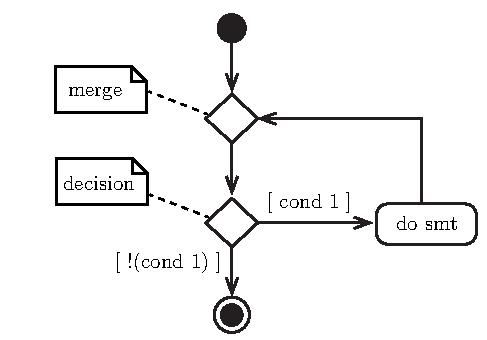
\includegraphics[width=0.50\linewidth]{01_Basics/figures/uml/IterationStatement-00-UML-while.pdf}
% \captionof{figure}{UML \texttt{while} Activity Diagram Representation}
% \label{fig:ch01_Basics_UML_IterationStatement-00-while}
% %~\ref{fig:ch01_Basics_UML_IterationStatement-00-while} 
% %%%%%%%%%%%%%%%%%%%%%%%%%%End figure
% \end{minipage}
% \begin{minipage}{.25\textwidth}
% %%%%%%%%%%%%%%%%%%%%%%%%%%%%%%%%%Begin code
% \begin{lstlisting}[frame=tlrb,numbers=none,mathescape=true,escapechar=\%,columns=flexible]
% some awesome code here
% \end{lstlisting}
% %%%%%%%%%%%%%%%%%%End Code
% \end{minipage}
% \vspace{0.5cm}
% %end minipages


%\begin{enumerate}
%	\item Initialize timer and directions registers
%    \item Specify initial state
%    \item Perform FSM controller
%   \begin{enumerate}
%    	\item Call an output function, which depends on the state
%        \item Delay, which depends on the state
%        \item Call an input function to get the status of the coin sensors
%        \item Change states, which dependes on the state and the input
%    \end{enumerate}
%\end{enumerate}

% \begin{enumerate}
% 	\item Current instruction is finished,
%     \item Eight registers are pushed on the stack,
%     \item LR is set to 0xFFFFFFF9,
%     \item IPSR is set to the interrupt number,
%     \item PC is loaded with the interrupt vector
% \end{enumerate}

% Itemize categoriza poniendo (.) en lugar de números
% \begin{itemize} 
% 	\item I
% 	\item I
% 	\item Y
% 	\item Y
% 	\item Y
% 	\item Y
% 	\item 
% \end{itemize}

% \begin{table}[!h]
% \centering
% \begin{tabular}{|l|l|l|} \hline
% $p$ & bit Field & Interrupt         \\\hline
% $3$ & \bitsRange[31]{29} & Interrupt [$4m+3$]  \\\hline
% $2$ & \bitsRange[23]{21} & Interrupt [$4m+2$]  \\\hline
% $1$ & \bitsRange[15]{13} & Interrupt [$4m+1$]  \\\hline
% $0$ & \bitsRange[7]{5} & Interrupt [$4m$]   \\\hline
% \end{tabular}
% \caption{pasteCaption}
% \label{tab:t_rt_ch04_}
% ~\ref{tab:t_rt_ch04_}
% \end{table}

% Insertar URL
%\url{https://www.osha.gov/Publications/laboratory/OSHAfactsheet-laboratory-safety-noise.pdf}\\

% \newcommand{\bitsRange}[2][50]{\texttt{{#1}-{#2}}}
% \newcommand{\CustomHex}[2][0000]{\texttt{0x{#1}.{#2}}}
% \newcommand{\GPIOPort}[1]{\texttt{GPIO\_PORT{#1}}}
% \newcommand{\GPIOPortR}[2][A]{\texttt{GPIO\_PORT{#1}\_{#2}\_R}}
% \newcommand{\GPIOPortHandler}[1]{\texttt{GPIO\_PORT{#1}\_Handler}}
% \newcommand{\HandlerISR}[1]{\texttt{#1\_Handler}}
% \newcommand{\IRQnr}[1]{\texttt{{#1}}}
% \newcommand{\NVICPRI}[1]{\texttt{NVIC\_PRI{#1}\_R}}
% \newcommand{\NVICEN}[1]{\texttt{NVIC\_EN{#1}\_R}}
% \newcommand{\NVICDIS}[1]{\texttt{NVIC\_DIS{#1}\_R}}
% \newcommand{\Ttimer}[2][A]{\texttt{Timer\_{#2}{#1}}}
% \newcommand{\xNrbit}[1]{$#1$-\texttt{bit}}
% \newcommand{\xNrbits}[1]{$#1$-\texttt{bits}}
% \newcommand{\camouflagegreenCellColor}{\cellcolor[rgb]{0.47, 0.53, 0.42}}
% \newcommand{\lavenderCellColor}{\cellcolor[rgb]{0.9, 0.9, 0.98}}
% \newcommand{\volties}[2][0]{$\si{{#1}\volt}_{#2}$}
% \newcommand{\volti}[1]{$\si{{#1}\volt}$}
% \newcommand{\voltiposi}[1]{$+\si{{#1}\volt}$}
% \newcommand{\voltinega}[1]{$-\si{{#1}\volt}$}